\chapter{Modely}
\label{chap:models}

V~sekcii \ref{sec:hmm-alignment} sme si zadefinovali pHMM pre zarovnávanie sekvencií (obr. \ref{fig:simple-model}).
V~našom riešení sme predstavili 2 modifikácie pôvodného pHMM na zakomponovanie dodatočnej informácie, pričom sme využili klasifikátory. V~oboch modeloch sú klasifikátory rovnaké, aj s~rovnakým postupom trénovania. Líši sa len trénovanie samotného pHMM a architektúra modelu.

\section[Model s~klasifikátorom ako emisiou]{Model s~klasifikátorom ako emisiou (Model A)}
\label{sec:model-clf}

Tento model vyzerá rovnako ako základný model, aj pravdepodobnosti prechodov zostanú, ale emisnú pravdepodobnosť sme nahradili výstupom z~klasifikátora.

\begin{figure}[htp]
    \centering
    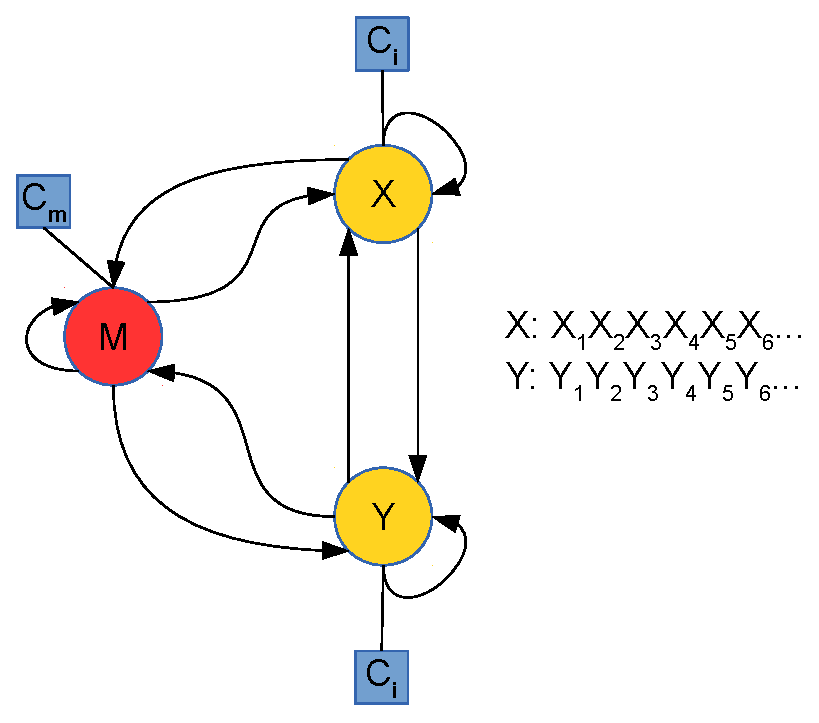
\includegraphics[width=.5\textwidth]{images/model_clf}
    \caption{Model s~klasifikátorom ako emisiou}
\end{figure}

Problémom tohto modelu je, že výstup klasifikátora nezodpovedá emisným pravdepodobnostiam, ale akejsi istote klasifikátora o~tom, že dve pozície majú byť zarovnané k~sebe. Hodnoty z~klasifikátora teda nesumujú do 1 a model nie je korektný pravdepodobnostný model. V~praxi sa však ukázalo (viď sekcia \ref{sec:cmp-model}), že to až tak nevadí, avšak o~takomto modeli už nemôžme hovoriť ako o~pravdepodobnostnom. Je len inšpirovaný pHMM.

\section[Model s~klasifikátorovou páskou]{Model s~klasifikátorovou páskou (Model B)}
\label{sec:model-tape}
(\todo alebo s~orákulom?)

Keďže predošlý model nie je korektný pravdepodobnostný model, navrhli sme alternatívny model, ktorý navyše modeluje aj výstup z~klasifikátora.
Nemodelujeme teda len dvojicu sekvencií, ale aj sekvenciu výstupov klasifikátora vo forme pásky. Tento model teda je korektný pravdepodobnostný model.
Pásku s~výstupom z~klasifikátora považujeme za akúsi pomôcku pre náš zarovnávač.

\begin{figure}[htp]
    \centering
    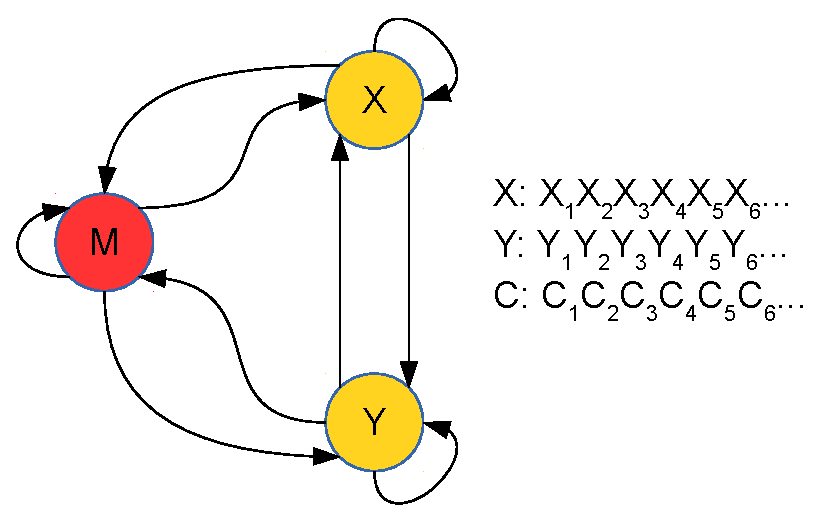
\includegraphics[width=.5\textwidth]{images/model_clf_paska}
    \caption{Model s~klasifikátorovou páskou}
\end{figure}

Keďže stále ide o~párový HMM, pásku si musíme predstaviť ako cestu v~2D tabuľke výstupov klasifikátorov, ktorá sa zhoduje s~cestou zarovnania. Teda ak sa pohneme horizontálne  alebo vertikálne, používame Indel klasifikátor a ak sa pohneme diagonálne tak použijeme Match klasifikátor.

\subsection{Diskrétna verzia}

Klasifikátor môže ľubovoľnú vrátiť hodnotu z~intervalu $\left<0,1 \right>$. Keďže výstup z~klasifikátora je spojitý, museli sme ho pre naše potreby diskretizovať.
Diskretizovať hodnoty môžme 2 spôsobmi, buď priamo -- spočítať histogram pre trénovacie dáta, alebo nepriamo -- interpolovať vstupnú vzorku pomocou spojitej distribúcie, napr. pomocou zmesi gausiánov a potom toto rozdelenie diskretizovať (obr. \ref{fig:clf-discretisation}). Druhá spomenutá metóda má výhodu v~tom, že vyhladí šum, ale treba s~ňou narábať opatrne, aby sme nezaviedli príliš veľkú nepresnosť. V~oboch prípadoch si musíme zvoliť počet košov $b$, do ktorých dáta rozdelíme. Koše sme rozdelili rovnomerne a na základe experimentov sme si zvolili $b = 10$.
% todo experimenty a porovnanie týchto 2 prístupov

\begin{figure}[htp]
        \centering
        \begin{subfigure}[c]{0.3\textwidth}
                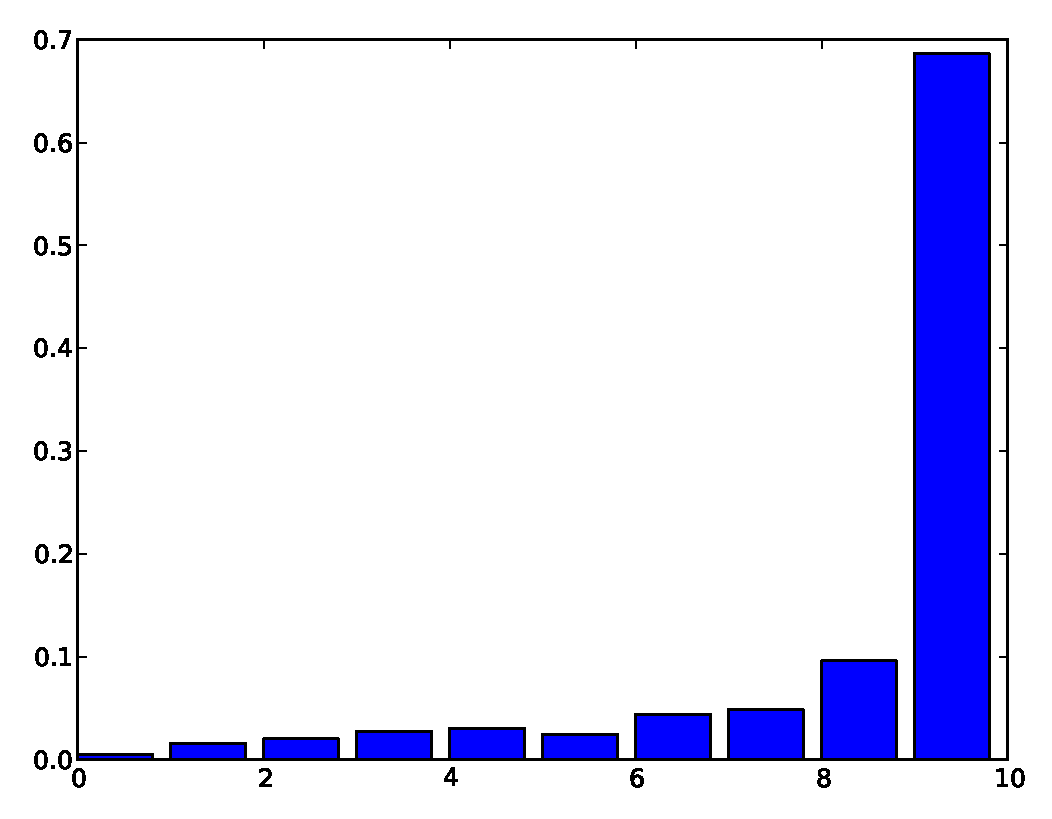
\includegraphics[width=\textwidth]{images/hist1}
                \caption{Histogram}
                \label{fig:clf-discretisation-1}
        \end{subfigure}%
        % \qquad\qquad %add desired spacing between images, e. g. ~, \quad, \qquad etc.
          %(or a blank line to force the subfigure onto a new line)
          % $\Rightarrow$
        $\vcenter{\hbox{\raisebox{.8cm}{\Huge\pointer}}}$
        \begin{subfigure}[c]{0.3\textwidth}
                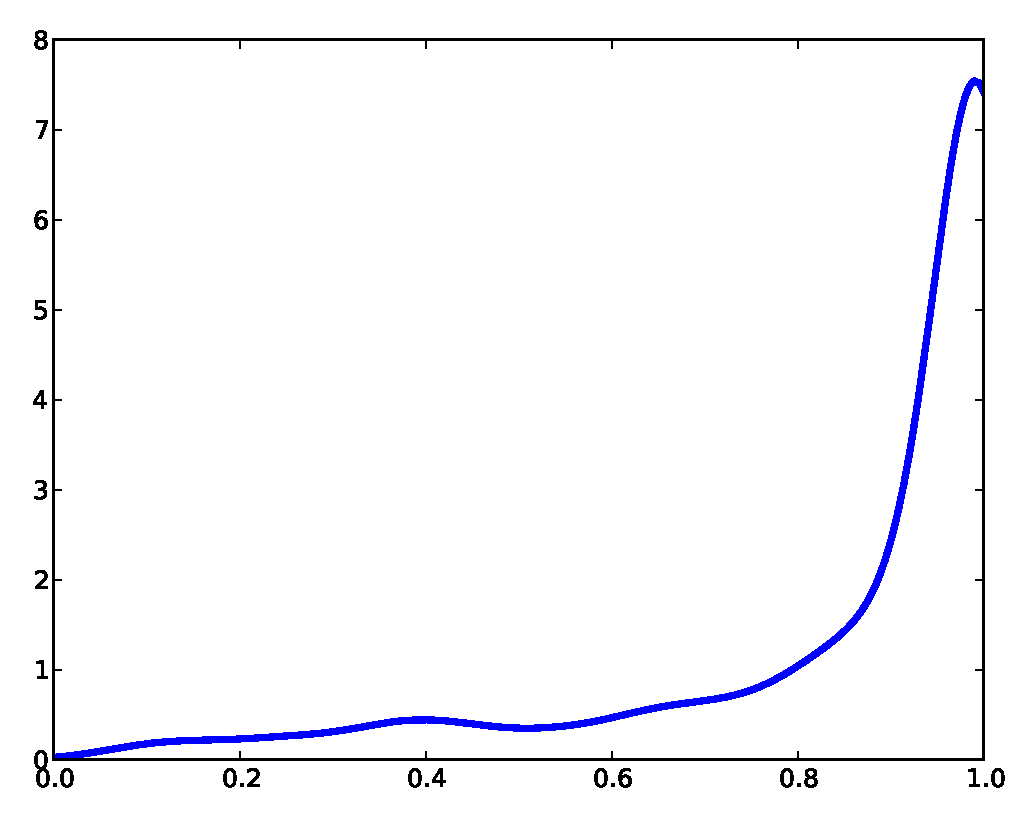
\includegraphics[width=\textwidth]{images/hist2}
                \caption{Zmes gausiánov}
                \label{fig:clf-discretisation-2}
        \end{subfigure}
        $\vcenter{\hbox{\raisebox{.8cm}{\Huge\pointer}}}$
        \begin{subfigure}[c]{0.3\textwidth}
                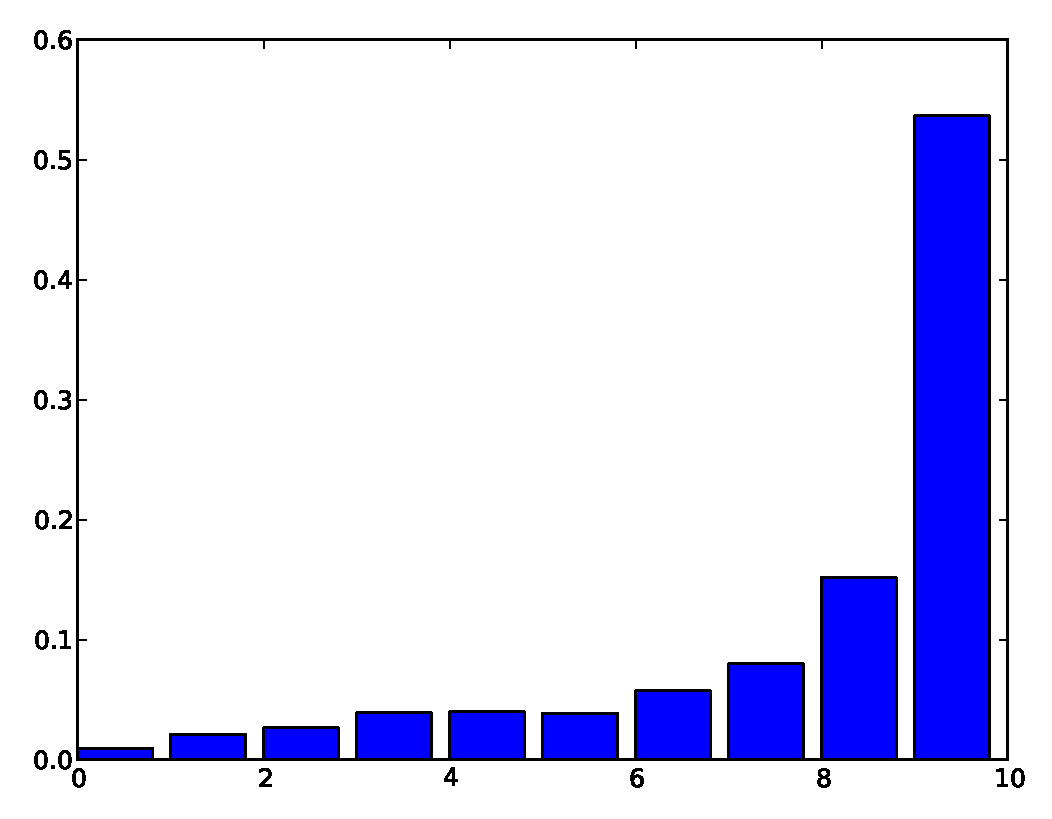
\includegraphics[width=\textwidth]{images/hist3}
                \caption{Nasekaný gausián}
                \label{fig:clf-discretisation-3}
        \end{subfigure}
        \caption[Diskretizácia výstupu klasifikátora]{Dve možnosti diskretizácie výstupu klasifikátora -- buď použijeme histogram \ref{fig:clf-discretisation-1}, alebo dáta najskôr aproximujeme pomocou zmesi gausiánov \ref{fig:clf-discretisation-2} a následne rozsekáme na koše \ref{fig:clf-discretisation-3}.}
        \label{fig:clf-discretisation}
\end{figure}

\subsection{Spojitá verzia}

Alternatíva k~predošlej metóde je použiť spojitý HMM. Hlavný rozdiel medzi spojitými a diskrétnymi HMM je, že spojité HMM nepočítajú s~pravdepodobnosťou, ale s~hustotou. Hodnota hustoty v~danom bode narozdiel od pravdepodobnosti môže byť aj väčšia ako jedna. Jedným zo štandardných spôsobov reprezentácie hustoty v~spojitých HMM je zmes gausiánov. \cite{huang1989multiple}, takže využijeme interpoláciu takouto distribúciou a to budeme brať ako hustotu výstupu klasifikátora (obr. \ref{fig:clf-discretisation-2}).

Ako vidíme z~tabuľky \ref{tab:success-b-tape}, spojitá verzia modelu sa nám neosvedčila. Má totiž nedostatok, že distribučná funkcia nedosahuje maximum pri výstupe klasifikátora rovnom jedna, ale kúsok predtým, čo znamená istú penalizáciu v~prípade, že si je klasifikátor príliš istý. To, či použijeme vyhladenie pomocou gausiánu až tak nezaváži, ale rozhodli sme sa ho predsa len využiť, pretože úspešnosť bola trochu vyššia takmer na všetkých testovaných sekvenciách.


\begin{table}[h]
\catcode`\-=12
\centering
\begin{tabular}{cc}
\toprule
& Úspešnosť\\
\midrule
Histogram & 82,25\%\\
Nasekaný gausián & 82,98\%\\
Zmes gausiánov & 65,59\%\\
\bottomrule
\end{tabular}
\vspace{0.5cm}
\caption[Porovnanie úspešností pri rôznom spracovaní pásky]{Porovnanie úspešností modelu B pri rôznom spracovaní pásky.}
\label{tab:success-b-tape}
\end{table}

\section{Trénovanie modelov}

\subsection{Trénovanie modelu A}

V~modeli~A~sme trénovali iba prechodové pravdepodobnosti, emisie sme mali priamo z~natrénovaného klasifikátora. Prechodové pravdepodobnosti sme trénovali pomocou metôdy maximálnej vierohodnosti, tak ako sme si to popísali v~kapitole \ref{subsec:hmmtraining}.

\subsection{Trénovanie modelu B}

V~modeli B sme trénovali aj tranzície aj emisie, opäť metôdou maximálnej vierohodnosti. Pri trénovaní emisií sme však urobili malú zmenu. Aby sme vedeli ľahko interpolovať vstupnú vzorku a~z~dôvodu lepšej vizualizácie sa nám hodí modelovať pravdepodobnosti $P(C|X \cap Y)$ (resp. $P(C|X)$ a $P(C|Y)$). Ukážeme si, že pravdepodobnosť $P(X \cap Y \cap C)$ vieme rozložiť pomocou $P(C|X \cap Y)$ a $P(X \cap C)$ vieme rozložiť pomocou $P(C|X)$.

$P(X \cap Y)$ poznáme z~frekvenčnej tabuľky a $P(C)$ vieme rozložiť pomocou nasledujúcej vety.

\begin{vt}[Veta o~úplnej pravdepodobnosti]
Nech $A_1\dots A_n$ tvoria rozklad univerza~$\Omega$ a nech $B$ je udalosť, potom
$$P(B) = \sum_{i=1}^n P(B|A_i)P(A_i)$$
\end{vt}

Máme teda
$$P\left[C=c\right] = \sum_{\forall x\in X, y \in Y} P\left[C=c | X=x \wedge Y=y\right] P\left[X=x \wedge Y=y\right],$$
pričom druhý člen poznáme a $P\left[C=c | X=x \wedge Y=y\right]$ už vieme ľahko dopočítať. Keď máme fixnuté dve bázy, vieme vybrať z~trénovacej sekvencie všetky pozície, kde sú zarovnané tieto bázy a vypočítať distribúciu C.

Pre Indel stav postupujeme analogicky, ibaže namiesto $P(X \cap Y)$ máme buď $P(X)$ alebo $P(Y)$ podľa toho, ktorý stav práve počítame.

Vieme teda pravdepodobnosť emisie $(x, y, c)$ Match stave vypočítať ako $$P\left[C=c \wedge X=x \wedge Y=y\right] = P\left[C=c | X=x \wedge Y=y\right] P\left[X=x \wedge Y=y\right]$$ a pravdepodobnosť emisie $(x, c)$ resp. $(y, c)$  v~Inzert stavoch pomocou
\begin{align*}
P\left[C=c \wedge X=x\right] &= P\left[C=c | X=x\right] P\left[X=x\right]\\
P\left[C=c \wedge Y=y\right] &= P\left[C=c | Y=y\right] P\left[Y=y\right].
\end{align*}
Emisie môžme teda natrénovať zvlášť pre každú dvojicu báz (resp. pre každú bázu).

\subsection{Popis trénovacej a testovacej množíny}

V~tejto sekcii sa budeme zaoberať len množinami pre trénovanie parametrov modelu. Množiny pre trénovanie klasifikátora sme si popísali v~kapitole \ref{subsec:clf-training-sets}.

V~prípade simulovaných dát 1 a 2 boli trénovacie množiny pre naše modely jedno zarovnanie dĺžky 10000. Testovacie množiny boli 6 zarovnaní dĺžky 1000. Zarovnania boli vygenerované našim simulátorom. V~tabuľke \ref{tab:sim-params} uvádzame pravdepodobnosť mutácie pre jednotlivé dáta.

\begin{table}
\centering
\begin{tabular}{cccc}
\toprule
anotácia $X$ & anotácia $Y$ & sim1 & sim2\\
\midrule
1 & 1 & 0,20 & 0,01\\
1 & 0 & \multirow{2}{*}{0,35} & \multirow{2}{*}{0,30}\\
0 & 1\\
0 & 0 & 0,40 & 0,99\\
\bottomrule
\end{tabular}
\caption[Pravdepodobnosť mutácie v~našich datasetoch]{Pravdepodobnosť mutácie v~simulovaných dátach 1 a 2}
\label{tab:sim-params}
\end{table}

\section{Výsledky experimentov}

\subsection{Porovnanie modelov}
\label{sec:cmp-model}
Hlavný rozdiel v~modeloch A~a B, ktoré sme predstavili v~sekciách \ref{sec:model-clf} a \ref{sec:model-tape} je v~tom, že prvý model je diskriminačný, zatiaľčo druhý je generatívny. (\todo mozno toto lepsie sformulovat alebo vyhodit lebo si nie som isty ci je to celkom pravda)

Model A~emituje len na základe natrénovaného klasifikátora, takže čokoľvek dokážeme klasifikátor naučiť, môžme priamo použiť. Model B používa klasifikátor iba ako pomôcku. Model funguje podobne ako štandardný model pre zarovnanie (sekcia \ref{subsec:hmm-alignment}) a klasifikátor iba mierne upravuje výsledné pravdepodobnosti.

\begin{table}
\centering
\begin{tabular}{ccc}
\toprule
bázy & výstup klasifikátora & emis. pravd.\\
\midrule
AA & 0.96 & 0,09399\\
AG & 0.96 & 0,00513\\
AA & 0.42 & 0,00729\\
AA & 0.26 & 0,00411\\
AG & 0.02 & 0,00168\\
\bottomrule
\end{tabular}
\caption[Porovnanie emisných pravdepodobností]{Porovnanie emisných pravdepodobností pre rôzne bázy a výstup natrénovaného klasifikátora}
\label{tab:emission-prob}
\end{table}

Ako môžme v~tabuľke \ref{tab:emission-prob} vidieť, pre rovnaký výstup klasifikátora, ale rôzne bázy sa emisná pravdepodobnosť môže líšiť. Dokonca aj pre značne nižší výstup klasifikátora pri rovnakých bázach môže byť pravdepodobnosť emisie stále vyššia ako pri rôznych bázach s~vysokým výstupom z~klasifikátora. Na druhej strane si môžme tiež všimnúť, že pri nižšom výstupe klasifikátora emisná pravdepodobnosť rapídne klesá a pri dostatočne nízkom výstupe klasifikátora pri rovnakých bázach už je emisná pravdepodobnosť nižšia, ako pri rôznych bázach s~vysokým výstupom klasifikátora.



\begin{table}[htp]
\todo pregenerovať s~oknom 9\\
\centering
\begin{tabular}{crrr}
\toprule
& Model A~& Model B & Ref. model\\
\midrule
Simulované 1 & 79,75\% & 84,35\% & 85,78\%\\
Simulované 2 & 72,62\% & 18,57\% & 6,78\% \\
\bottomrule
\end{tabular}

\caption[Porovnanie úspešností modelov]{Porovnanie úspešností modelov. Referenčný model je obyčajný pHMM na zarovnávanie DNA sekvencií. Úspešnosť je počítaná ako percentuálna zhoda originálneho a nového zarovnania. Simulované dáta 1 sa snažia napodobňovať biologické procesy, Simulované dáta 2 nezodpovedajú biologickým dátam a sú zložitejšie na natrénovanie pre referenčný model.}
\label{tab:success-compare}
\end{table}

V~tabuľke \ref{tab:success-compare} sme porovnávali, ako sa modely dokážu prispôsobiť zložitejším dátam. Môžme si všimnúť, že model A~sa správa konzistentne na oboch typoch dát, zatiaľ čo model B sa pri zložitejšom type dát nechal stiahnuť dole nutnosťou dodržovať pravdepodobnosti generovania báz.

\subsection{Rôzne veľkosti okna}

V~tejto sekcii sme sa venovali hľadaniu optimálnej veľkosti okna. Vyskúšali sme viacero možností a výsledky sme zapísali do tabuľke \ref{tab:window-compare}.

\begin{table}[htp]
\centering
\begin{tabular}{ccc}
\toprule
Veľkosť okna & Model A~& Model B\\
\midrule
1 & 76,95\% & 57,86\%\\
3 & 70,62\% & 81,42\%\\
5 & 73,95\% & 82,98\%\\
7 & 78,31\% & 83,05\%\\
9 & 79,75\% & 84,35\%\\
11 & 79,28\% & 83,57\%\\
13 & 80,58\% & 83,98\%\\
15 & 81,62\% & 83,98\%\\
\bottomrule
\end{tabular}
\caption[Porovnanie úspešností pri rôznej veľkosti okna]{Porovnanie úspešností modelov pri rôznej veľkosti okna.}
\label{tab:window-compare}
\end{table}

Z~tabuľky vidíme, že pre model B je optimálna veľkosť okna 7-9, pri väčších oknách už úspešnosť nerastie. Pri modeli A~rástla úspešnosť až po veľkosť okna 15. Optimálnu hodnotu pre model A~sme na základe tabuľky určili na 9-15.

\subsection{Vplyv dodatočnej informácie na zarovnanie}

V~tejto sekcii sme zisťovali, aký vplyv má dodatočná informácia na zarovnanie. Vyskúšali sme zakázať anotácie pri veľkosti okna jedna a 9. Pri veľkosti okna rovnej jedna nemáme okrem anotácie žiadnu ďalšiu informáciu. Pri veľkosti okna 9 máme aj okolie sekvencie.

\begin{table}[htp]
\centering
\begin{tabular}{cccc}
\toprule
Veľkosť okna & Anotácia & Model A~& Model B\\
\midrule
1 & nie & 74,42\% & 18,35\%\\
1 & áno & 76,95\% & 57,86\%\\
9 & nie & 78,43\% & 82,67\%\\
9 & áno & 79,75\% & 84,35\%\\
\bottomrule
\end{tabular}
\caption[Vplyv dodatočnej informácie na zarovnanie]{Vplyv dodatočnej informácie na zarovnanie.}
\label{tab:annotation-compare}
\end{table}

V~tabuľke \ref{tab:annotation-compare} si môžme všimnúť, že zatiaľ čo pri modeli A~je úspešnosť veľmi podobná, hoci aj anotácie aj väčšie okno mierne pomohli. Naopak pri modeli B sú rozdiely výrazne väčšie, vidíme, že aj samotná anotácia výrazne pomohla a väčšie okno je pre tento model nutnosťou.

\subsection{Použitie jedného klasifikátora pre Match aj Inzert stav}

V~tejto sekcii sme vyskúšali nahradenie Indel klasifikátora Match klasifikátorom, ktorý vracia opačné hodnoty. Teda trénujeme len jeden klasifikátor.

\begin{table}[htp]
\centering
\begin{tabular}{ccc}
\toprule
 & Model A~& Model B\\
\midrule
1 klasifikátor & 74,53\% & 82,72\%\\
2 klasifikátory & 79,75\% & 84,35\%\\
\bottomrule
\end{tabular}
\caption[Porovnanie použitia jedného alebo dvoch typov klasifikátorov]{Porovnanie použitia jedného alebo dvoch typov klasifikátorov.}
\label{tab:1clf-compare}
\end{table}

Z~tabuľky \ref{tab:1clf-compare} vidno, že použitie dvoch typov klasifikátorov má svoje opodstatnenie, hoci naše modeli dokášu fungovať aj z~jedným.

\subsection{Porovnanie modelov s~existujúcimi zarovnávačmi}

V~tejto sekcii sme porovnali naše výsledky s~výsledkami referenčného modelu a zarovnávača \textit{muscle} \cite{edgar2004muscle}.

\begin{table}[htp]
\catcode`\-=12
\centering
\begin{tabular}{lcccccccc}
\toprule
\multirow{2}{*}{Dáta} &
\multicolumn{2}{c}{Model A} &
\multicolumn{2}{c}{Model B } &
\multicolumn{2}{c}{Ref. Model } &
\multicolumn{2}{c}{Muscle} \\
\cmidrule(r){2-3}\cmidrule(lr){4-5}\cmidrule(lr){6-7}\cmidrule(l){8-9}
& Zhoda & Tranz. & Zhoda & Tranz. & Zhoda & Tranz. & Zhoda & Tranz.\\
\midrule
Simulované 1 & 79,75\% & 44,97\% & 84,35\% & 56,5\% & 85,78\% & 61,03\%\\
Simulované 2 &  & & \\
Biologické &  & & \\
\bottomrule
\end{tabular}
\caption[Porovnanie s~existujúcimi zarovnávačmi]{Porovnanie našich modelov s~referenčným modelom a zarovnávačom muscle.}
\label{tab:window-compare}
\end{table}

\section{Zhrnutie}
